% ================================================================
% ================================================================
% --- PREAMBLE
% --- Document class
\documentclass[12pt]{article}

% --- Packages
\usepackage[utf8]{inputenc}
\usepackage[top=1in, bottom=1in, left=1in, right=1in]{geometry}
\usepackage{setspace}
\usepackage{microtype}
\usepackage[dvipsnames]{xcolor}
\usepackage{lastpage}
\usepackage{hyperref}
\usepackage{fancyhdr}
\usepackage{booktabs}
\usepackage{graphicx}
\usepackage{todonotes}
\usepackage{fontspec}
\usepackage[backend=biber, style=apa, citestyle=apa]{biblatex}

% --- Settings
%\setmainfont{Caladea}
\usepackage{libertine}
\usepackage[libertine]{newtxmath}
\addbibresource{references.bib}

\hypersetup{
    colorlinks = true,
    linkcolor  = blue,
    urlcolor   = blue,
    citecolor  = blue,
    }
    
\pagestyle{fancy}

% --- Header and footer
\fancyhf{}
\headheight = 28pt
\chead{20 YEARS OF DOLLARIZATION IN ECUADOR\\
       \textit{Nicolás Cachanosky and John Ramseur}}
\cfoot{\footnotesize Page \thepage \hspace{0.5pt} of \pageref{LastPage}} 

% --- Title page
\title{20 YEARS OF DOLLARIZATION IN ECUADOR: A SYNTHETIC CONTROL ANALYSIS
       \thanks{We appreciate comments by Lawrence H. White. Any error or omission is our own.} \\
       \bigskip}

\author{
        \textbf{Nicolás Cachanosky} \\
        Metropolitan State University of Denver \\
        Department of Economics \\
        \href{mailto:ncachano@msudenver.edu}{ncachano@msudenver.edu} \\
        \and
        \textbf{John Ramseur} \\
        Metrpolitan State University of Denver \\
        Department of Economics \\
        \href{mailto:jramseur@msudenver.edu}{jramseur@msudenver.edu} \\
        \bigskip}

\date{\today}


% ================================================================
% ================================================================
% --- DOCUMENT
\setlength{\marginparwidth}{2cm}
\begin{document}


% ================================================================
% --- TITLE PAGE

\maketitle

\begin{abstract}
\noindent
This paper uses a Synthetic Control Analysis to examine the economic effectiveness of dollarization in Ecuador. We address common concerns surrounding the adoption of dollarization as a policy and provide several solutions to those concerns. We find that dollarization resulted in significant higher levels of income without clear evidence of worsening in social health variables such as infant mortality, poverty, and income distribution.
\end{abstract}

\bigskip \bigskip
\footnotesize \noindent \textbf{JEL codes}: E42; E50; O43 \\
\footnotesize \noindent \textbf{Keywords}: Ecuador, dollarization, synthetic control analysis

\newpage
\doublespacing


% ================================================================
% --- SECTION 1: INTRODUCTION
\section{Introduction} 
    \label{sec:intro}

Twenty years ago, in 2000, Ecuador dollarized its economy in the middle of an inflationary crisis. The case of Ecuador is relevant for other countries with troubled currencies, such as Argentina or Venezuela. Besides also being located in Latin America, Ecuador is a larger economy in the region, providing a different case study to those of small dollarized economies such as El Salvador or Panamá. 

The benefits and costs of dollarization was a debated topic at the turn of the century, when Ecuador and Argentina followed different path. The former dollarized its economy. The latter refused the option and faced one of its largest economic crisis in 2001. Despite the major reform that dollarization entails, policy discussion remained mostly speculative. 

Even though history offers more than hundred cases of dollarization \parencite{Schuler2005}, usable data for typical regression analysis remains limited. Maybe this is a reason why the discussion surrounding dollarization has remained highly speculative \parencite[for a sample see][]{Levy-Yeyati2002,Salvatore2003}. Sachs and Larrain \parencite*{Sachs1999} offer a good representation of those who oppose to dollarization arguing that it is a "reckless" (p. 80) straitjacket. Yet, other scholars consider that dollarization can be a good reform for countries with troubled currencies  \parencite{Avila2018,Cochrane2018,Gale2002,Hanke2003a,White2014a} 

Previous work on Ecuador's dollarization looks at issues such as the loss of seigniorage \parencite{Lange2005}, its effects on fiscal policy \parencite{MariDelCristo2016}, or how feasible it is to de-dollarize Ecuador \parencite{JAMESON2003}. In addition, Jansen and Ortiz \parencite*{Jansen2007} find that the probability of large negative returns in stocks decreased post dollarization while that of positive returns increased. This paper complements the studies on Ecuador's dollarization with the novel application of a synthetic control analysis (SCA) \parencite{Abadie,Abadie2003,Abadie2015}. This method allows building the counterfactual of a non-dollarized synthetic-Ecuador. By doing this, we can compare how the economy of dollarized Ecuador compares with the economy of had Ecuador not dollarized. We find that GDP per capita of dollarized Ecuador outperforms the would-be GDP per capita of non-dollarized Ecuador.\footnote{In recent years, SCA has been applied in a number of different studies. For instance, Rok \parencite*{Spruk2019} studies the economic cost of institutional shocks to Argentina; Grier and Maynard \parencite*{Grier2016} and Absher, Grier, and Grier \parencite*{Absher2020} study market reforms in Georgia; and Powell, Clark, and Nowrasteh \parencite*{Powell2017} look at the impact of mass immigration in Israel.}

The paper proceeds in the following way. Section 2 reviews the dollarization debate. Section 3 presents an overall view of economic and social series for Ecuador. Section 4 develops the SCA analysis. Section 5 concludes.

% ================================================================
% --- SECTION 2: THE DOLLARIZATION DEBATE: MAIN CONCERNS
\section{The Dollarization Debate}
    \label{sec:debate}

Dollarization is the adoption of a foreign currency by a domestic country whether the currency adopted is the U.S. dollar (USD), the New Zealand dollar, the Euro, the British Pound, or any other foreign currency. Dollarization can either by unilateral or bilateral. In the former case, the dollarizing country unilaterally decides to adopt a foreign currency. In the latter, there is an agreement with the central bank that can include, for instance, sharing some of the new seigniorage that dollarization will bring.

Another issue to consider is that dollarization can also be either formal or informal. In the former case, the government formally adopts a foreign currency, while in the latter case economic agents decide to use a foreign currency regardless of the government's mandate. The distinction between formal and informal dollarization is important because it draws a distinction between a spontaneous and planned dollarization reforms. In the first case we have a bottom-up institutional change spontaneously driven by the private sector. In the second case we have a top-down government reform. Ecuador represents a bottom-up dollarization in the sense that it was the public who chose to use the USD and later on the government decided to formalize such decision \parencite{White2014a}. It was not the government who imposed the USD on the public, it was the public who imposed the USD on the government.\footnote{For a more detailed analysis if Ecuador's dollarization see Beckerman and Solimano \parencite*{Beckerman2002}.}

As mentioned before, the dollarization debate has been highly speculative. The debate can be summarized in four issue: (1) the problem of loosing monetary policy, (2) the problem of the absence of a lender of last resort (LOLR), (3) the problem of loosing seigniorage, and (4) the problem of unnecessary dollarization by its necessary conditions.

% --- SUB-SECTION 2.1
\subsection{The Problem of Losing Monetary Policy}

When a country dollarizes it gives up the possibility of executing its own domestic monetary policy. Some critics argue that this lack of control serves as a restrictive straitjacket rather than as reform that liberates the country from its own inefficient monetary policy \parencite{Sachs1999}. This constraint is particularly important in the case of foreign nominal shocks that would require a prudent and well calibrated reaction by a domestic central banks. Sachs and Larrain \parencite[][p. 80]{Sachs1999}, they describe dollarization as a "reckless" reform.

However, the point of dissent is not a dollarized economy will be unable to carry its own monetary policy. The point of dissent is whether dollarization, despite all its shortcomings, is a better alternative to an erratic domestic central bank. The whole point of dollarization is to shut down the domestic central bank because its a constant source of nominal shocks and high inflation.

It is unclear that in countries that face a potential dollarization domestic monetary policy is as independent as it is assumed to be. A detachment from foreign nominal shocks requires the adoption of a free floating exchange rate. However, many developing countries suffer from feat of floating  \parencite{Calvo2002}, which means that in practice the domestic central bank is deviating from the ideal domestic strategy. If domestic monetary policy is going to be reticent to devalue when facing foreign shocks, then it is unclear what benefit the domestic country is giving up by dollarizing. In other words, the alleged benefit of a domestic central bank is inversely related with the degree of fear of floating.\footnote{Levy-Yeyati, Sturzenegger, and Gluzmann \parencite{Levy-Yeyati2003} argue that some countries face more fear of appreciation than of depreciation.}

Furthermore, a cost-benefit analysis of dollarization must avoid falling into the Nirvana fallacy \parencite{Demsetz1969}. Objecting to dollarization on the grounds that the ideal domestic monetary policy will be unfeasible is a Nirvana fallacy type of argument. Countries that face a potential dollarization do not have ideal central bank, they have very inefficient ones. The realistic choice is between dollarization and a central bank unable to commit to efficiency.

For the purpose of framing the discussion, consider the following Taylor-rule reaction function of the domestic central bank.\footnote{This policy reaction is presented just for illustration purposes. A country that faces a potential dollarization is in such monetary disorder that the central bank may not follow any reaction policy other than a day-to-day decision about how to make it to the next day.}

\begin{equation} \label{Eq:1}
    i_t = i^*_t + \phi_\pi \tilde{\pi}_t + \phi_X \tilde{X}_t + \varepsilon_t
\end{equation}

where $t$ is the time period, $i$ and $i^*$ denote short-term and short-term equilibrium interest rates, $\tilde{\pi}$ is the inflation gap, $\tilde{X}$ is the gap of other variables (such as output or unemployment gap), $\phi$ are positive numbers and $\varepsilon$ is an error term or shock. A deviation form the interest rate dictated by the policy rule would produce economic costs, such a deviation from the inflation target, misallocation of resources, relative price distortion, monetary illusion, and so on.

The main concern is dollarization is exposed to negative shock (a large negative $\varepsilon$) that could lead the economy into a serious recession. In terms of equation \ref{Eq:1}, the alternative is not a domestic central bank that produces small deviations from the policy rule. The alternative is a domestic central bank being the source of large values of $\varepsilon$. The efficient central bank is not a feasible option; otherwise dollarization wouldn't be necessary. Consider the case of Ecuador itself, between 1983 and its dollarization in 2000, the average yearly inflation rate was 42.2-percent. Argentina has a worse situation. Between the rise of Perón in 1946 and 2020, the yearly average inflation rate is 62-percent. Large shocks can originate externally and also internally. Far from being a settled issue, comparing the costs of domestic and external monetary shocks is an empirical question.

% --- SUB-SECTION 2.2
\subsection{The Problem of the Absence of a Lender of Last Resort}

A dollarized economy does not have a central bank to perform the duties of a LOLR. This is problematic because the financial market is seen as inherently unstable. According to this view, illiquid (yet solvent) banks are prone to suffer a bank run. If the bank run spreads through the financial market, then a LOLR is needed to get the situation under control and avoid a major financial crisis. For the purpose of this paper, we take the inherent instability of the banking sector as given.\footnote{The inherent instability view of banks rests on the Diamond and Dybvig \parencite*{Diamond1983}. For a critical review of this model and its implications see Cachanosky \parencite*[][Ch. 1]{Cachanosky2018a}, Dowd \parencite*{Dowd1992a}, Selgin \parencite*[][Ch. 11]{Selgin1996c}, and White \parencite*[][Ch. 6]{White1999c}.}

Using Bagehot's rule as a reference, a LOLR should lend only at a premium rate only to illiquid but solvent banks. A central bank can deviate from this rule, leading to moral hazard problems. As long commercial banks expect the central bank to offer bailout to insolvent banks, then said banks will be inclined to invest in riskier assets increasing the likelihood of a financial crisis. To avoid moral hazard, a central banks adherence to Bagehot's rule must be credible. This is not easy because central banks can bailout as many banks as desired without suffering losses or going bankrupt. In these terms, dollarization can be seen as a credible commitment to not bailout banks at the cost of not being able to do so when needed \parencite{Gale2002}. The credibility reading of dollarization is relevant for countries where central banks presidents do not face incentives to increase credibility due to their short term in office.\footnote{For instance, the Argentine central bank had 23 presidents between 1983 and 2015, with an average of 570 days in office.}

Yet, a LOLR can take many forms, a central bank being one of them. Therefore, dollarization does not mean there will be no LOLR, it means this role will not be performed by the monetary authority. One option is what Ecuador does, which is having a special tax on deposits to fund a liquidity fund that can be used if needed \parencite{Quispe-Agnoli2006}. This fund can be managed by a public office (as is the case of Ecuador) or by a consortium of private banks with the incentive to bailout only solvent banks. Another options is to mandate a deposit insurance.\footnote{The case of the United States is telling. Bank failures decreased with the implementation of the FDIC, not with the establishment of the Federal Reserve in 1913. See Selgin, Lastrapes, and White \parencite*[][pp. 582-583]{Selgin2012a}.} A third case would be to allow a deep integration with international financial markets, as is the case of Panamá \parencite{MorenoVillalaz1999,MorenoVillalaz2005}. Banks operating domestically can be owned by foreign banks, which would have the motivation and information to keep their international branches in a good financial situation. There is also the option of regulating reserve requirements and credit diversification. In short, the option is not between a LOLR (central bank) and no LOLR (dollarization). A range of different version of a LOLR are available. What is needed is an entity able to lend, not necessary one that can "print" its own money \parencite{Calvo2001}. Even a central bank with the capacity to create money may be limited on its role as LOLR if domestic banks and firms hold debt in foreign currency because the domestic currency inflates at a high rate.

The more private-market oriented a LOLR is, the closer it will adhere to Bagehot's rule minimizing moral hazard. A privately managed fund risks facing loses if it saves banks that are insolvent, but a central bank doe not face the same cost-benefit incentives. The underlying issue in the case of dollarization is not whether or not to have a LOLR, but what type of LOLR should be in place.\footnote{Bagehot's rule was endorsed by Ben Bernanke when serving as Chairman of the Federal Reserve. It is less clear that the acts of the Fed followed this endorsement \parencite{Hogan2015b}.}

% --- SUB-SECTION 2.3
\subsection{The Problem of Lost Seigniorage}

The decision to dollarize also means to give up seigniorage. Seigniorage is the revenue accruing to the currency issuer. Seigniorage must be distinguished from the inflation tax, which the extraction of the public's purchasing power by the government. The distinction between these two sources of revenue is important. In a well functioning economy, seigniorage is larger than the inflation tax. Differently, a country facing a potential dollarization may have negative seigniorage while collecting inflation tax.

The central bank's revenue is the interest collected by holding foreign-denominated assets. The central bank acquires these assets through open market operations. As long as its fiat currency is demanded by the market, the central bank can create its currency and buy foreign assets. The costs of the central bank are the interest rate it must pay for the market to hold its currency (for instance, issuing interest-bearing bonds) plus any operational cost.

\begin{equation}\label{Eq:2}
    S = ei^FA - iB - C
\end{equation}

where $S$ is the central bank seigniorage, $e$ is the nominal exchange rate, $i^F$ is the foreign nominal interest rate, $A$ is the amount of foreign assets, $i$ is the domestic interest rate paid by the central bank, $B$ is the amount of bonds issued by the central bank, and $C$ denote the operational costs of the monetary authority.

If there is high inflation, then the low demand for the domestic currency means the central bank must pay a high value of $iB$, potentially producing a negative seigniorage. The more informally dollarized an economy is, and the higher the inflation rate is, the less seigniorage the government collects.

What a dollarizing economy resigns to is the inflation tax. The inflation tax is typically regressive and highly distorting. Also, as a non-legislated tax it can be at odds with constitutional mandates. High inflation is not only economically costly, it can also contribute to institutional degradation. For a country facing an out of control inflation, giving up the inflation tax may be a low price to pay to get monetary stability.

Yet, some seigniorage can be kept domestically after a unilateral dollarization by adding some financial reforms. Following the examples of Scotland, Ireland and Hong Kong, domestic banks can be allowed to issue their own convertible banknotes \parencite[see][]{Hogan2012}. Seigniorage will be collected by the private sector rather than the government. The alternative, however, is the government collecting an inflation tax, not proper seigniorage from its central bank.

% --- SUB-SECTION 2.4
\subsection{The Problem of Unnecessary Dollarization by its Necessary Conditions}

Dollarization is not a reform intended to solve all of the economic problems of a country. Other reforms such as balancing the budget, deregulate the labor market, or remove trade restrictions are some examples of what else a country in need of dollarization should do. The need of other reforms begs if dollarization is still needed. If all these reforms are carried out, why dollarize? Seems that the necessary reforms to make dollarization robust and useful make it unnecessary at the same time. Dollarization is unnecessary by its own necessary reforms.

Dollarization can still be useful in two ways. The first one is being the trigger that makes the other reforms happen. Dollarization may be unneeded if other reforms take place, but these other reforms may not take place without dollarization. Dollarization may be unneeded with other reform in place, but dollarization is needed for those reforms to take place. The second one requires to avoid again a Nirvana fallacy type of argument. Certainly, if the feasible reforms are the ideal one, dollarization would not be needed. Yet, the feasible reforms may be enough for dollarization to work even if they are not idea. In that case, dollarization works as an institutional constrain on the government. Dollarization is not just a monetary policy reform, it is also an institutional reform. The credibility that the dollarizing country cannot produce is imported from a foreign country. 

Figure \ref{fig:Fig01} assumes that institutional quality ranks from 0 (worse) to 100 (best or ideal). Assume further that the institutional quality of a country considering dollarization is 40. Dollarization needs an institutional quality of 70 to be sustainable and beneficial, and becomes unnecessary with an institutional quality of at least 90. The realistic institutional reform this country can produce would produce an institutional quality of 80; more than what is necessary for dollarization to work, less than what would make it unnecessary.

\begin{figure}[h]
    \caption{Institutional reform and dollarization}
    \centering
    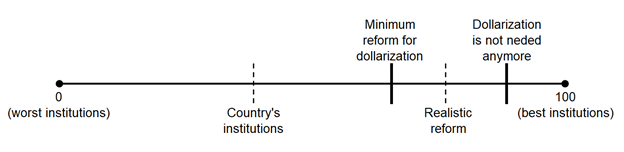
\includegraphics{Fig_01.png}
    \label{fig:Fig01}
\end{figure}

The institutional robustness of dollarization should not be underestimated. Dollarization in Ecuador survived (1) the left-leaning populist regime of Rafael Correa, (2) a sovereign debt default, (3) the 2008 financial crisis. Arguably, dollarization served as a constrain on populist policies. Absher, Grier, and Grier \parencite*{Absher2020} find that durable left-populist regimes in Latin America produce significant losses in real income. The only exception in their study is Ecuador, which is also the only dollarized country in their study.


% ================================================================
% --- SECTION 4: SYNTHETIC CONTROL ANALYSIS
\section{Synthetic Control Analysis}

\subsection{The SCA Method and Donor Pool Selection Criteria}

\subsection{Real GDP per Capita (PPP)}

\subsection{Export share of GDP}

\subsection{Infant Mortality}



% ================================================================
% --- SECTION 5: CONCLUSIONS


% ================================================================
% --- SECTION 6: REFERENCES
\newpage
\singlespacing
\printbibliography


% ================================================================
% --- THE END
\end{document}
